\documentclass{report}
\usepackage{amsmath}
\usepackage{graphicx}
\graphicspath{ {./} }
\begin{document}
\part{Question One}
\section{Question}
We want to combine three transformations into one by multiplying them. The transformation S should be applied second; the transformation T should be applied first; the transformation R should be applied third. Write the product of the three transformations showing the order in which they should be multiplied.
\section{Answer}
\begin{enumerate}
	\item Translation
	\item Scaling
	\item Rotation
\end{enumerate}
$\begin{bmatrix}
x^1 \\
y^1 \\
z^1
\end{bmatrix}
=
\underset{Translation}{\begin{bmatrix}
1 & 0 & 0 & a \\
0 & 1 & 0 & b \\
0 & 0 & 1 & c \\
0 & 0 & 0 & 1
\end{bmatrix}}
\underset{Scaling}{\begin{bmatrix}
a & 0 & 0 & 0 \\
0 & b & 0 & 0 \\
0 & 0 & c & 0 \\
0 & 0 & 0 & 1
\end{bmatrix}}
\underset{Rotation}{\begin{bmatrix}
\cos\theta & -a\sin\theta & 0 & 0 \\
\sin\theta & \cos\theta & 0 & 0 \\
0 & 0 & 1 & 0 \\
0 & 0 & 0 & 1
\end{bmatrix}}
\begin{bmatrix}
x \\
y \\
z \\
1 \\
\end{bmatrix}
\\
\begin{bmatrix}
a & 0 & 0 & a \\
0 & b & 0 & b \\
0 & 0 & c & c \\
0 & 0 & 0 & 1
\end{bmatrix}
\begin{bmatrix}
\cos\theta & -a\sin\theta & 0 & 0 \\
\sin\theta & \cos\theta & 0 & 0 \\
0 & 0 & 1 & 0 \\
0 & 0 & 0 & 1
\end{bmatrix}
\begin{bmatrix}
x \\
y \\
z \\
1 \\
\end{bmatrix}
\\
\underset{ResultingMatrix}{\begin{bmatrix}
\cos\theta & -a\sin\theta & 0 & a \\
\sin\theta & \cos\theta & 0 & b \\
0 & 0 & 1 & c \\
0 & 0 & 0 & 1
\end{bmatrix}
\begin{bmatrix}
x \\
y \\
z \\
1 \\
\end{bmatrix}}
$
\part{Question Two}
\section{Question}
Write the code that carries out the following steps. You may assume that the appropriate imports have been provided.
\section{Answer}
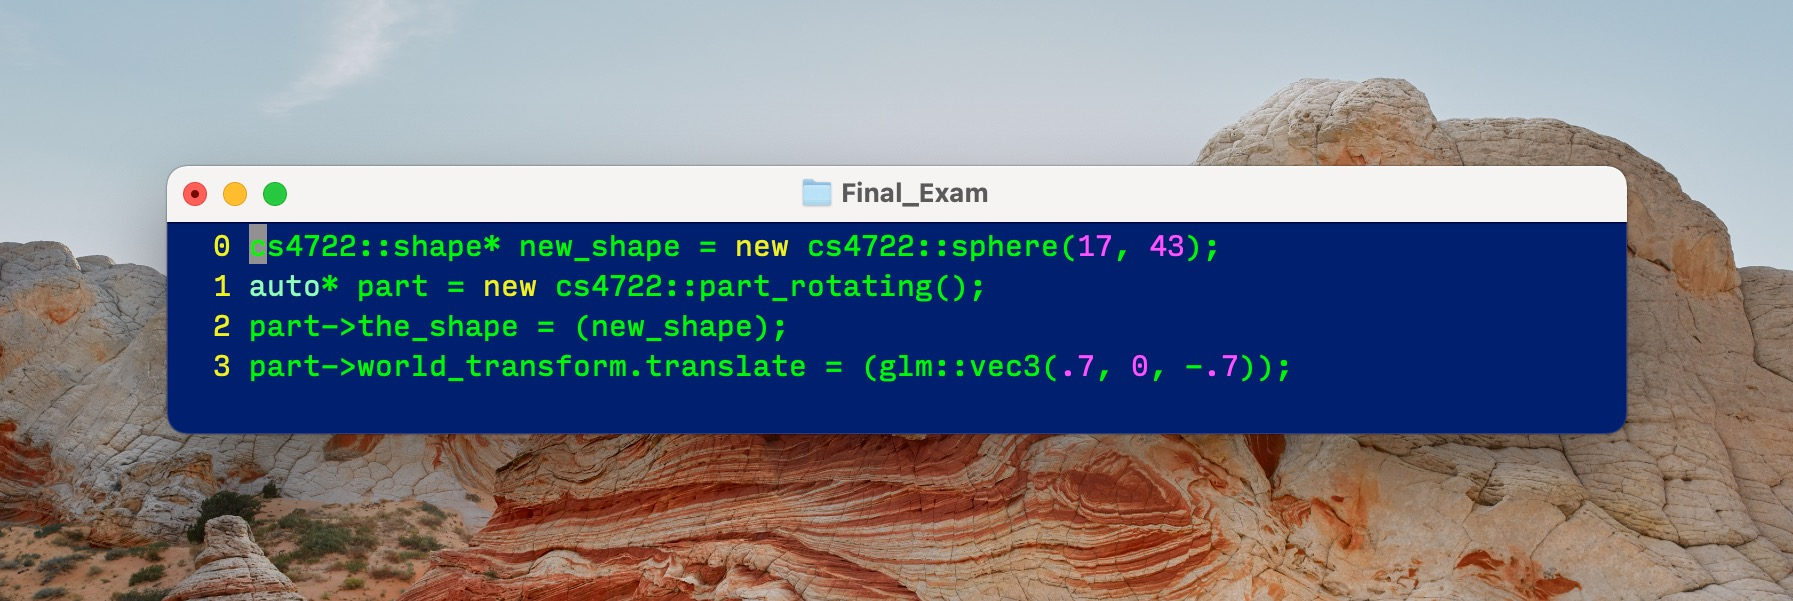
\includegraphics[width=1.0\textwidth]{question_two}
\part{Question Three: Data Memory}
\section{Question}
We want to render a geometric figure which is modeled using 38 triangles.
As with almost all of our examples, he figure will be drawn using gl triangles mode. This question is about measuring the memory used to store the vertex data.
\subsection{ How many vertices will be used to represent each triangle?}
\subsection{Answer}
3 Vertices will be used to represent each of the triangles using the gl triangles mode.
\subsection{ Using the standard way we have represented vertex positions in our code examples, how many float values will be used to represent each vertex position?
}
\subsection{Answer}
There will be four float values used with each of the vertex positions.
\subsection{ How many float values in all will it take to represent all the vertex positions for the figure?
}
\subsection{Answer}
It will take 456 float values to represent the 38 triangles.
\subsection{ How many bytes will that take to store all this position data?
}
\subsection{Answer}
It will take 1,824 Bytes to store all the position data in this scene.
\subsection{ In the examples where colors were assigned to vertices, each color was represented by a cs4722::color object. How many bytes does it take to store the data (r, g, b, and a components) of a cs4722::color object?}
\subsection{Answer}
There is one byte for each color coordinate, Given the R, G, B, and Components that will amount to four bytes.
\subsection{ How many bytes would it take to store all of the color data assigned to the vertices of this figure?}
\subsection{Answer}
Given that each color component is four bytes it will take 456 bytes of data for color storage in this scene.
\part{Question Four: Pipeline}
\section{Question}
Each part below describes a stage or a process in the standard OpenGL rendering pipeline. Your answer is to name the pipeline stage or process.
\subsection{ For a single geometric primitive, determines the pixels that are covered by the primitive.}
\subsection{Answer}
Primitive Setup
\subsection{ Subdivides shapes more complex than primitives into standard primitive shapes}
\subsection{Answer}
Culling and clipping
\subsection{ For a single vertex, does some processing and outputs a vertex to the later stages}
\subsection{Answer}
Vertex Shader
\subsection{ Takes one or more vertices and creates a geometric primitive from them}
\subsection{Answer}
Geometry Shader
\subsection{ For a single pixel, does some processing and outputs a color for that pixel}
\subsection{Answer}
Fragment Processing
\part{Question Five: Drawing Modes}
\section{Question}
The image to the below shows six points stored in the GPU buffer. The list of points starts with the black point, lower left, and continue around clockwise: black, red, green, blue, magenta, cyan. These points can be used to draw triangles or lines or points' in various ways, depending on the drawing mode. TRIANGLES or LINES for example.- -> For each picture below, tell which drawing mode was used to produce that picture. Each of the seven drawing modes available is used in one of the parts.
\subsection{POINTS}
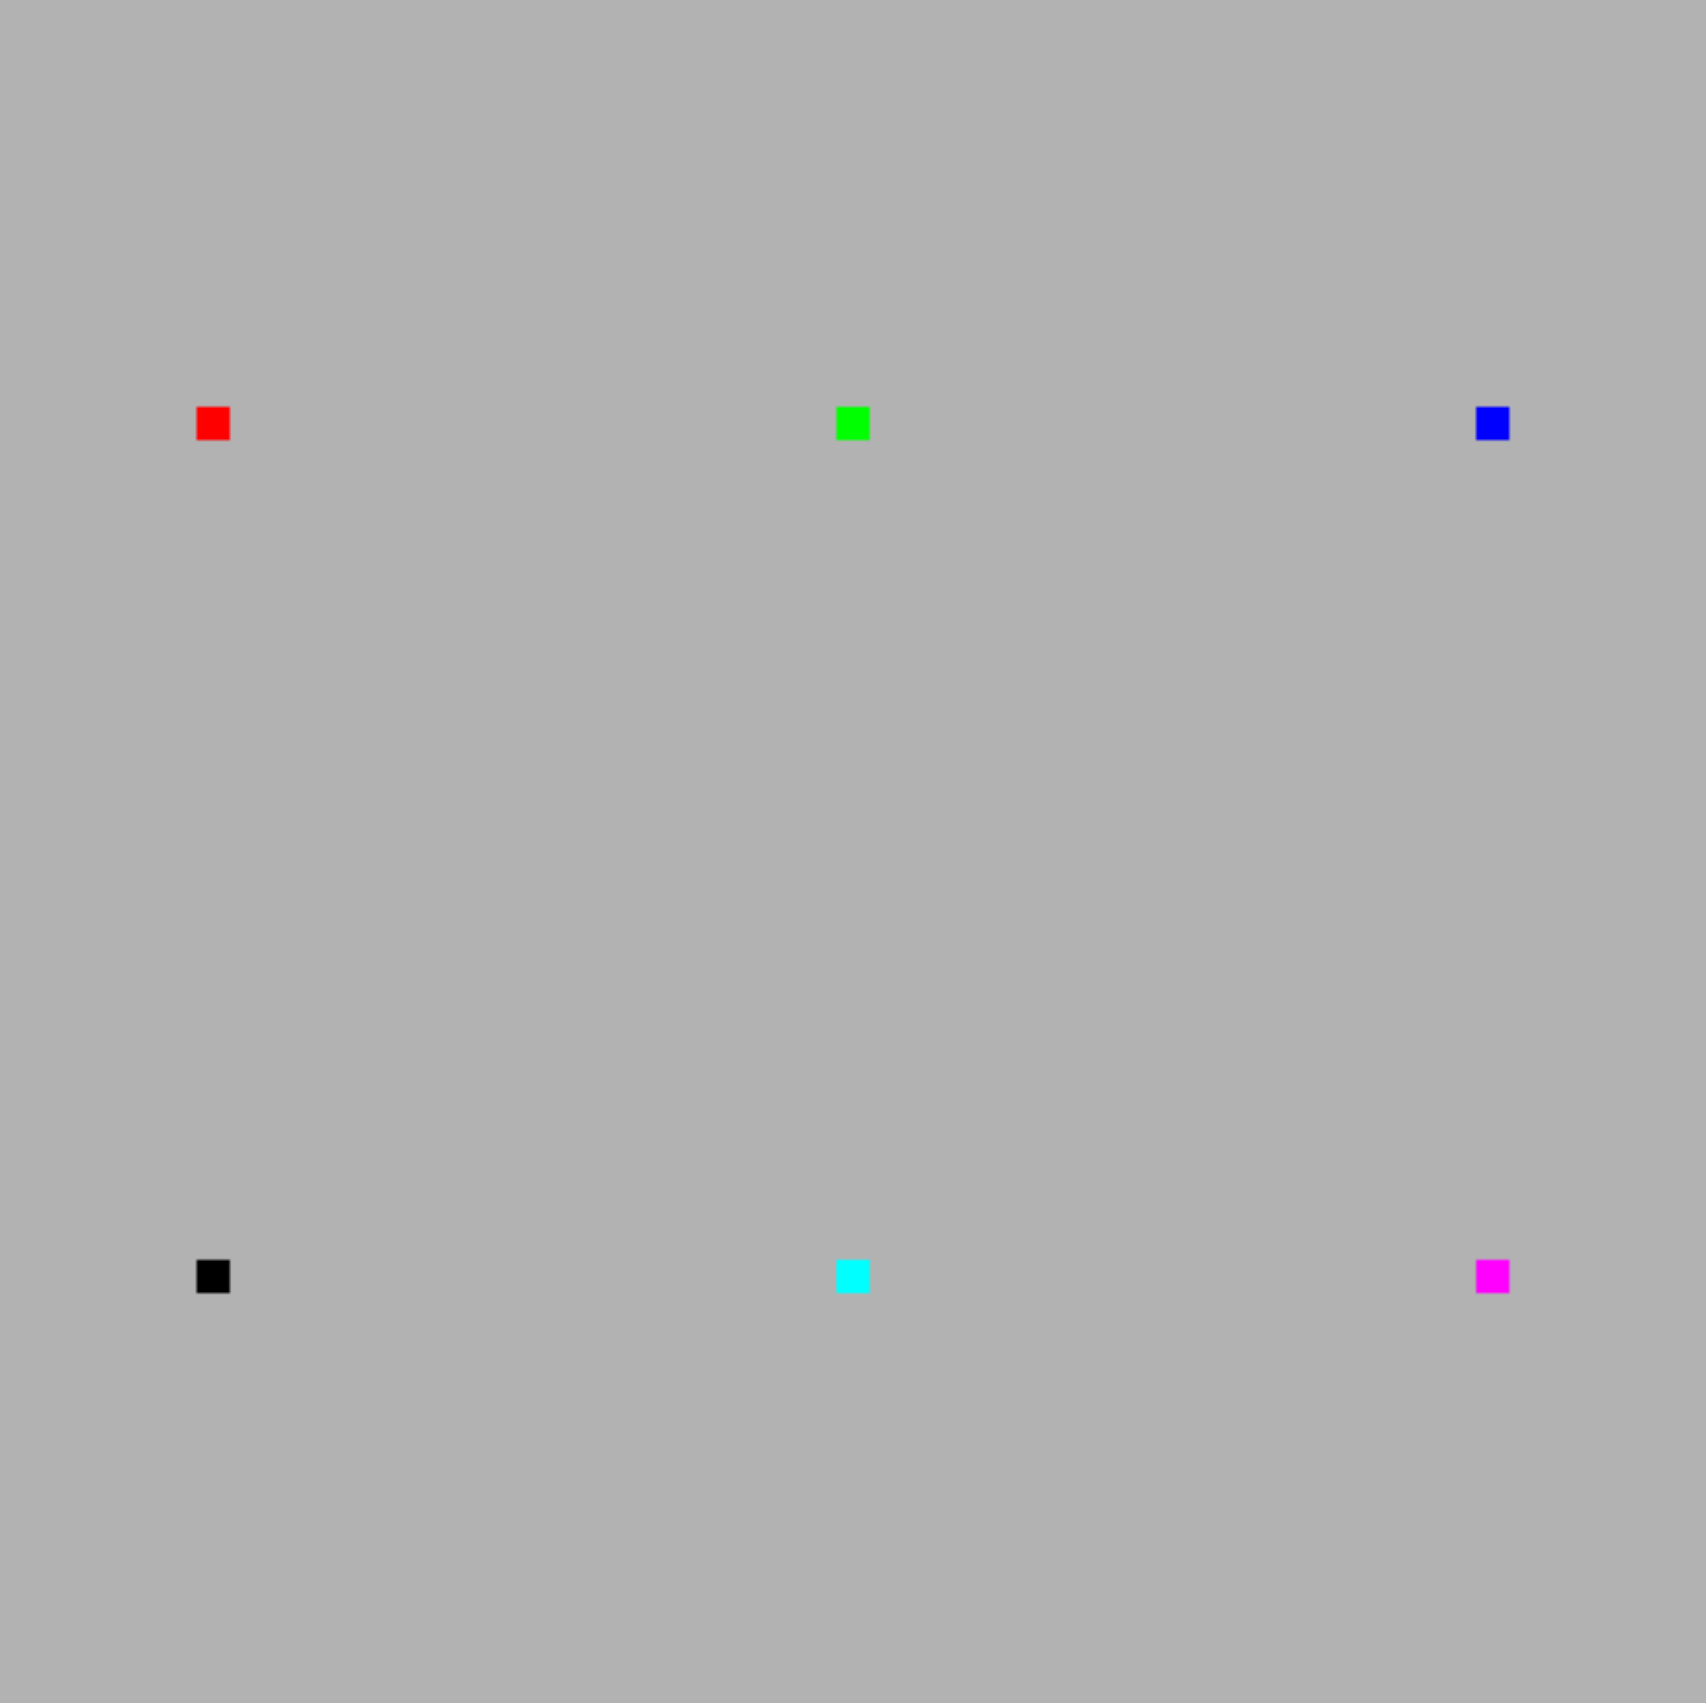
\includegraphics[width=1.0\textwidth]{Image_1}
\subsection{LINE STRIP}
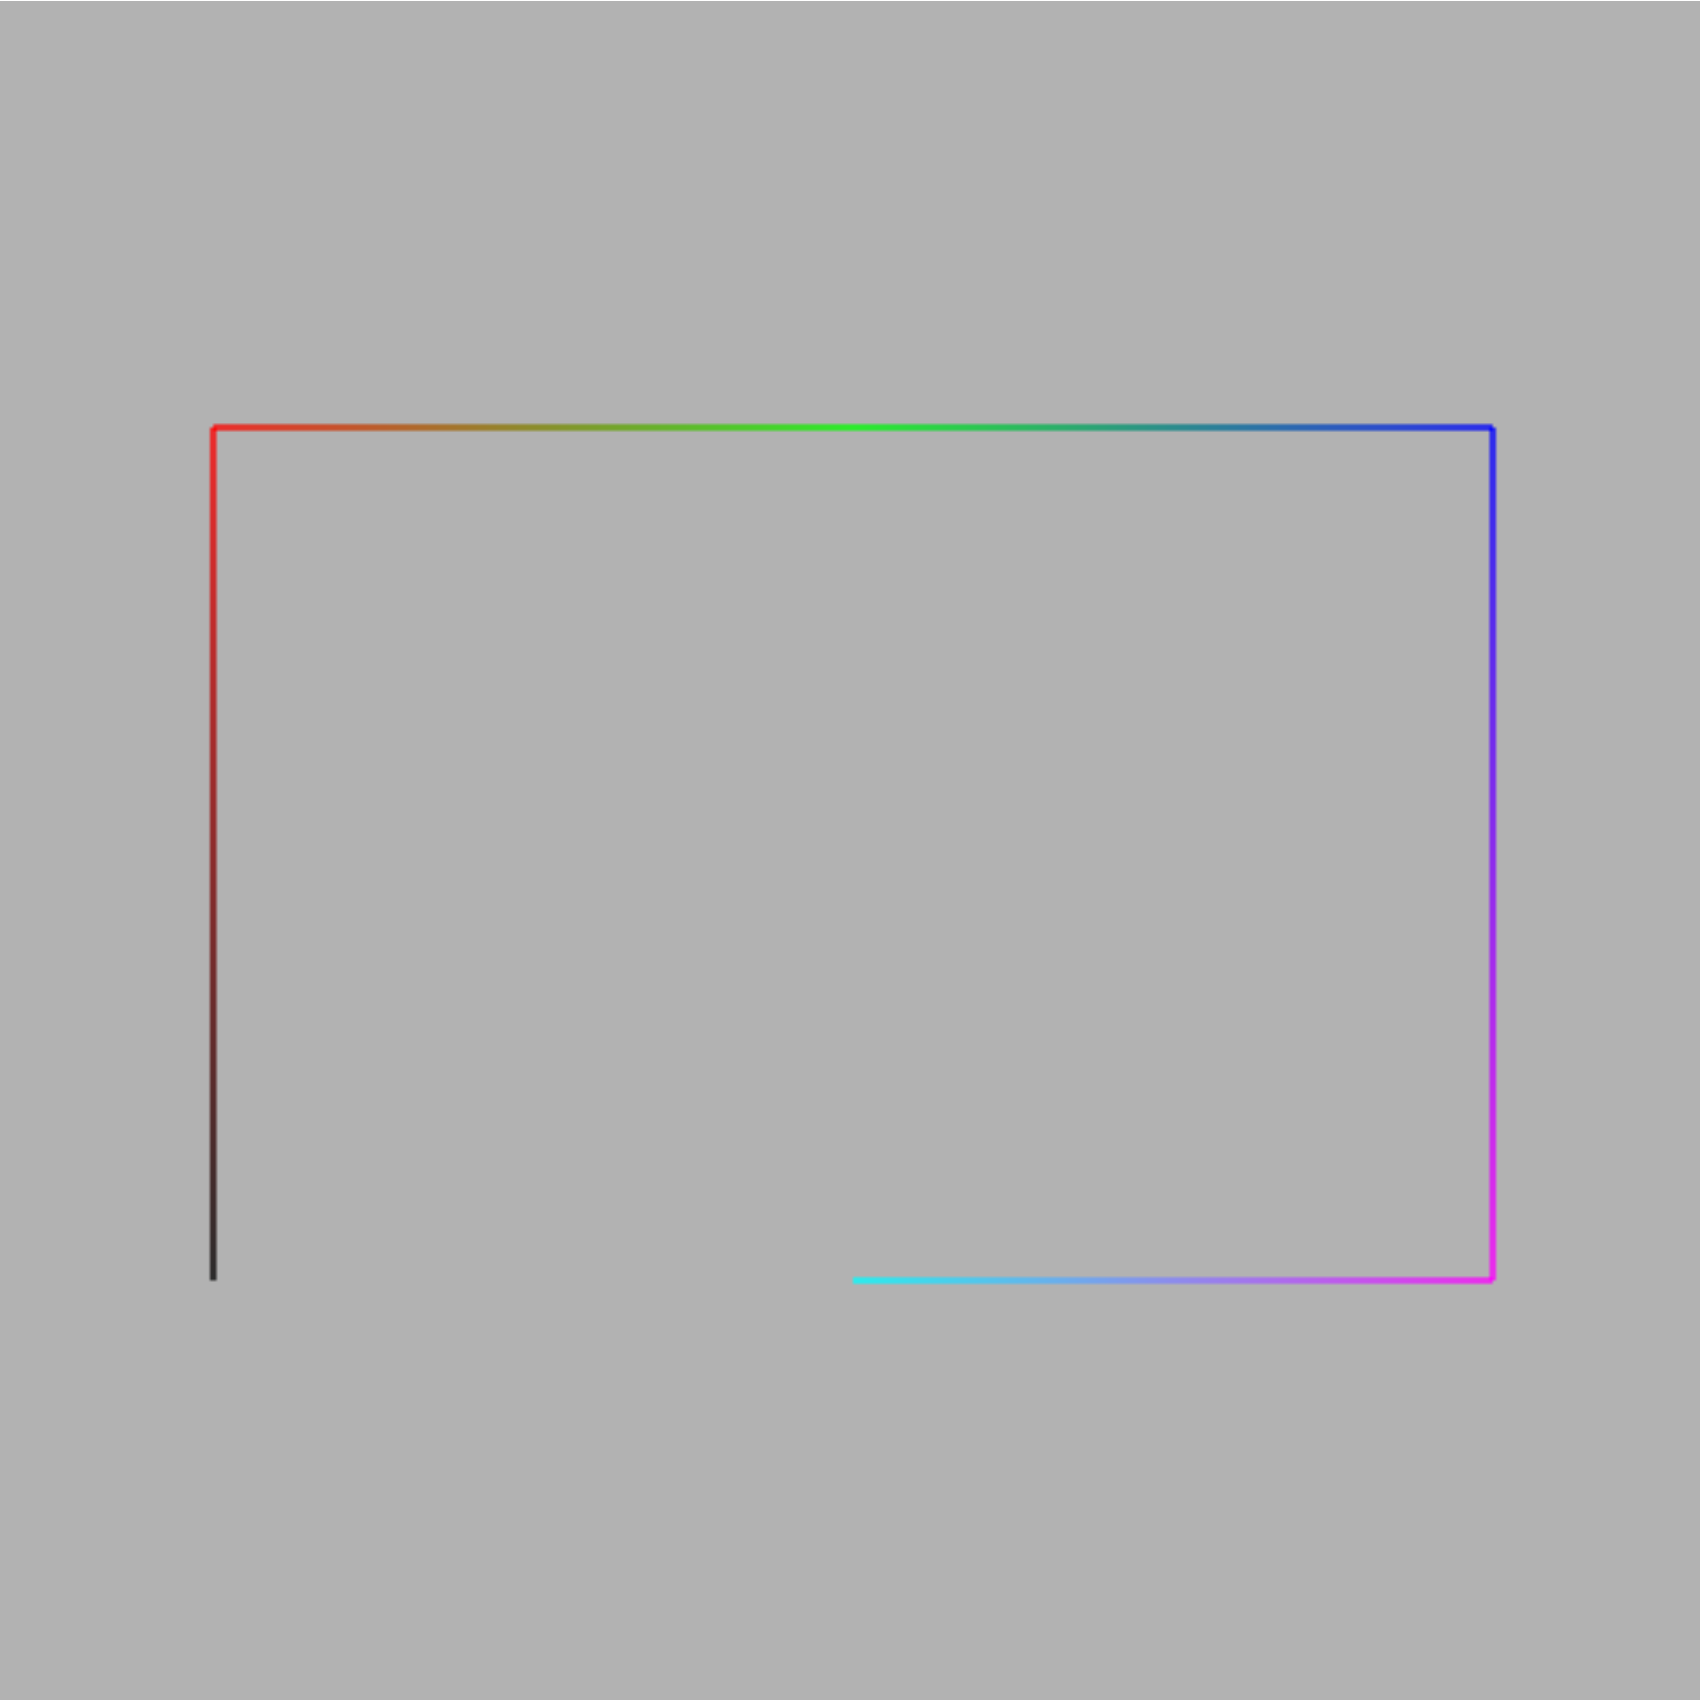
\includegraphics[width=1.0\textwidth]{Image_0}
\subsection{LINE LOOP}
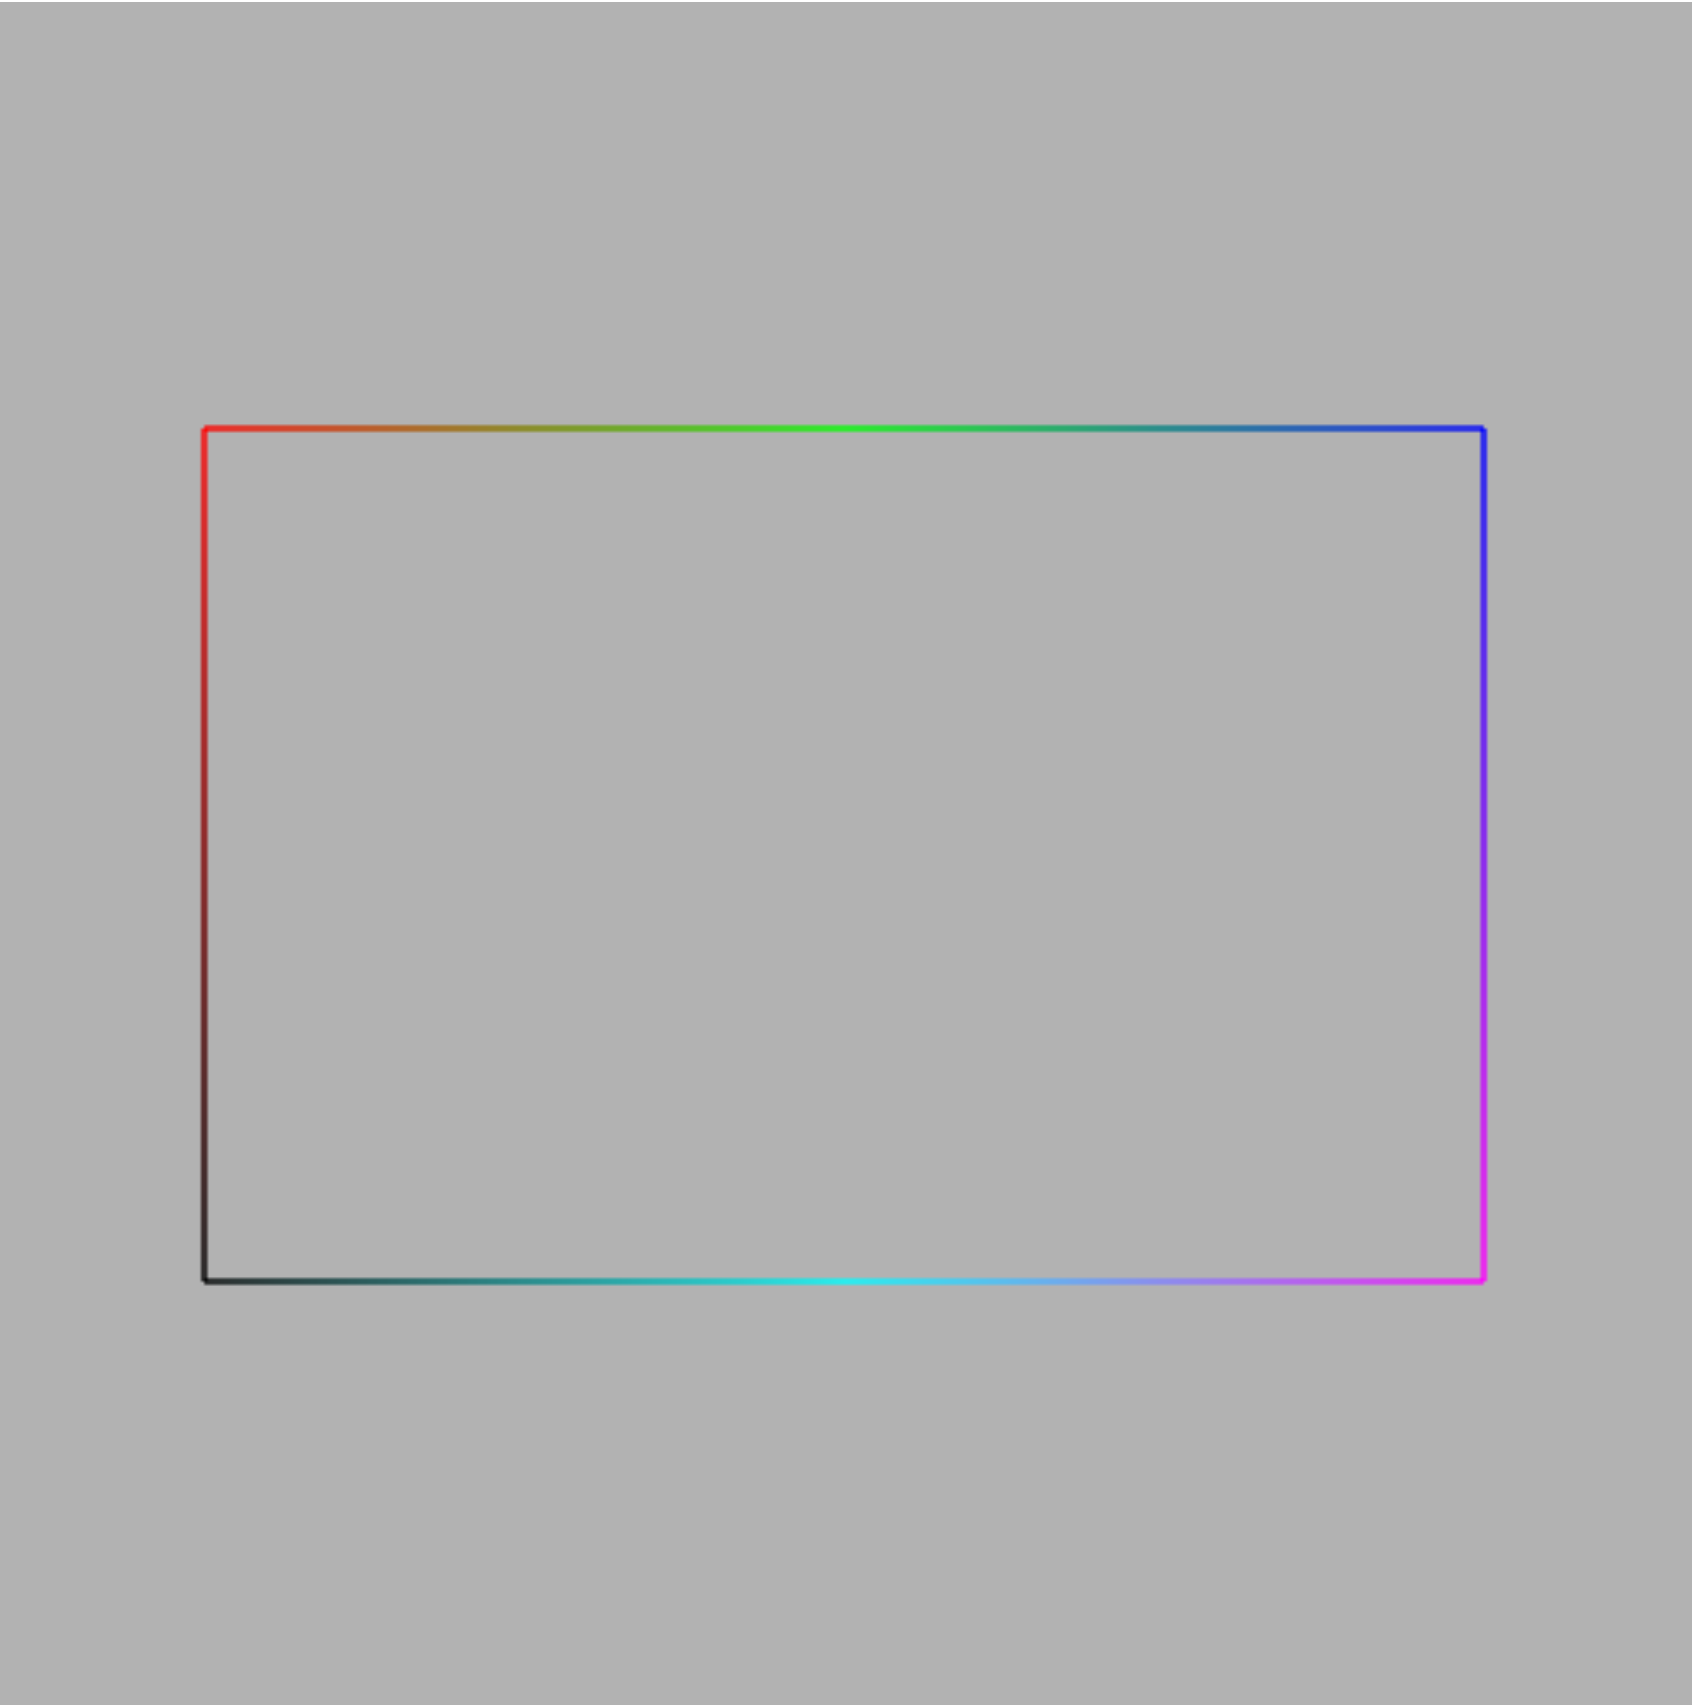
\includegraphics[width=1.0\textwidth]{Image_2}
\subsection{TRIANGLE STRIP}
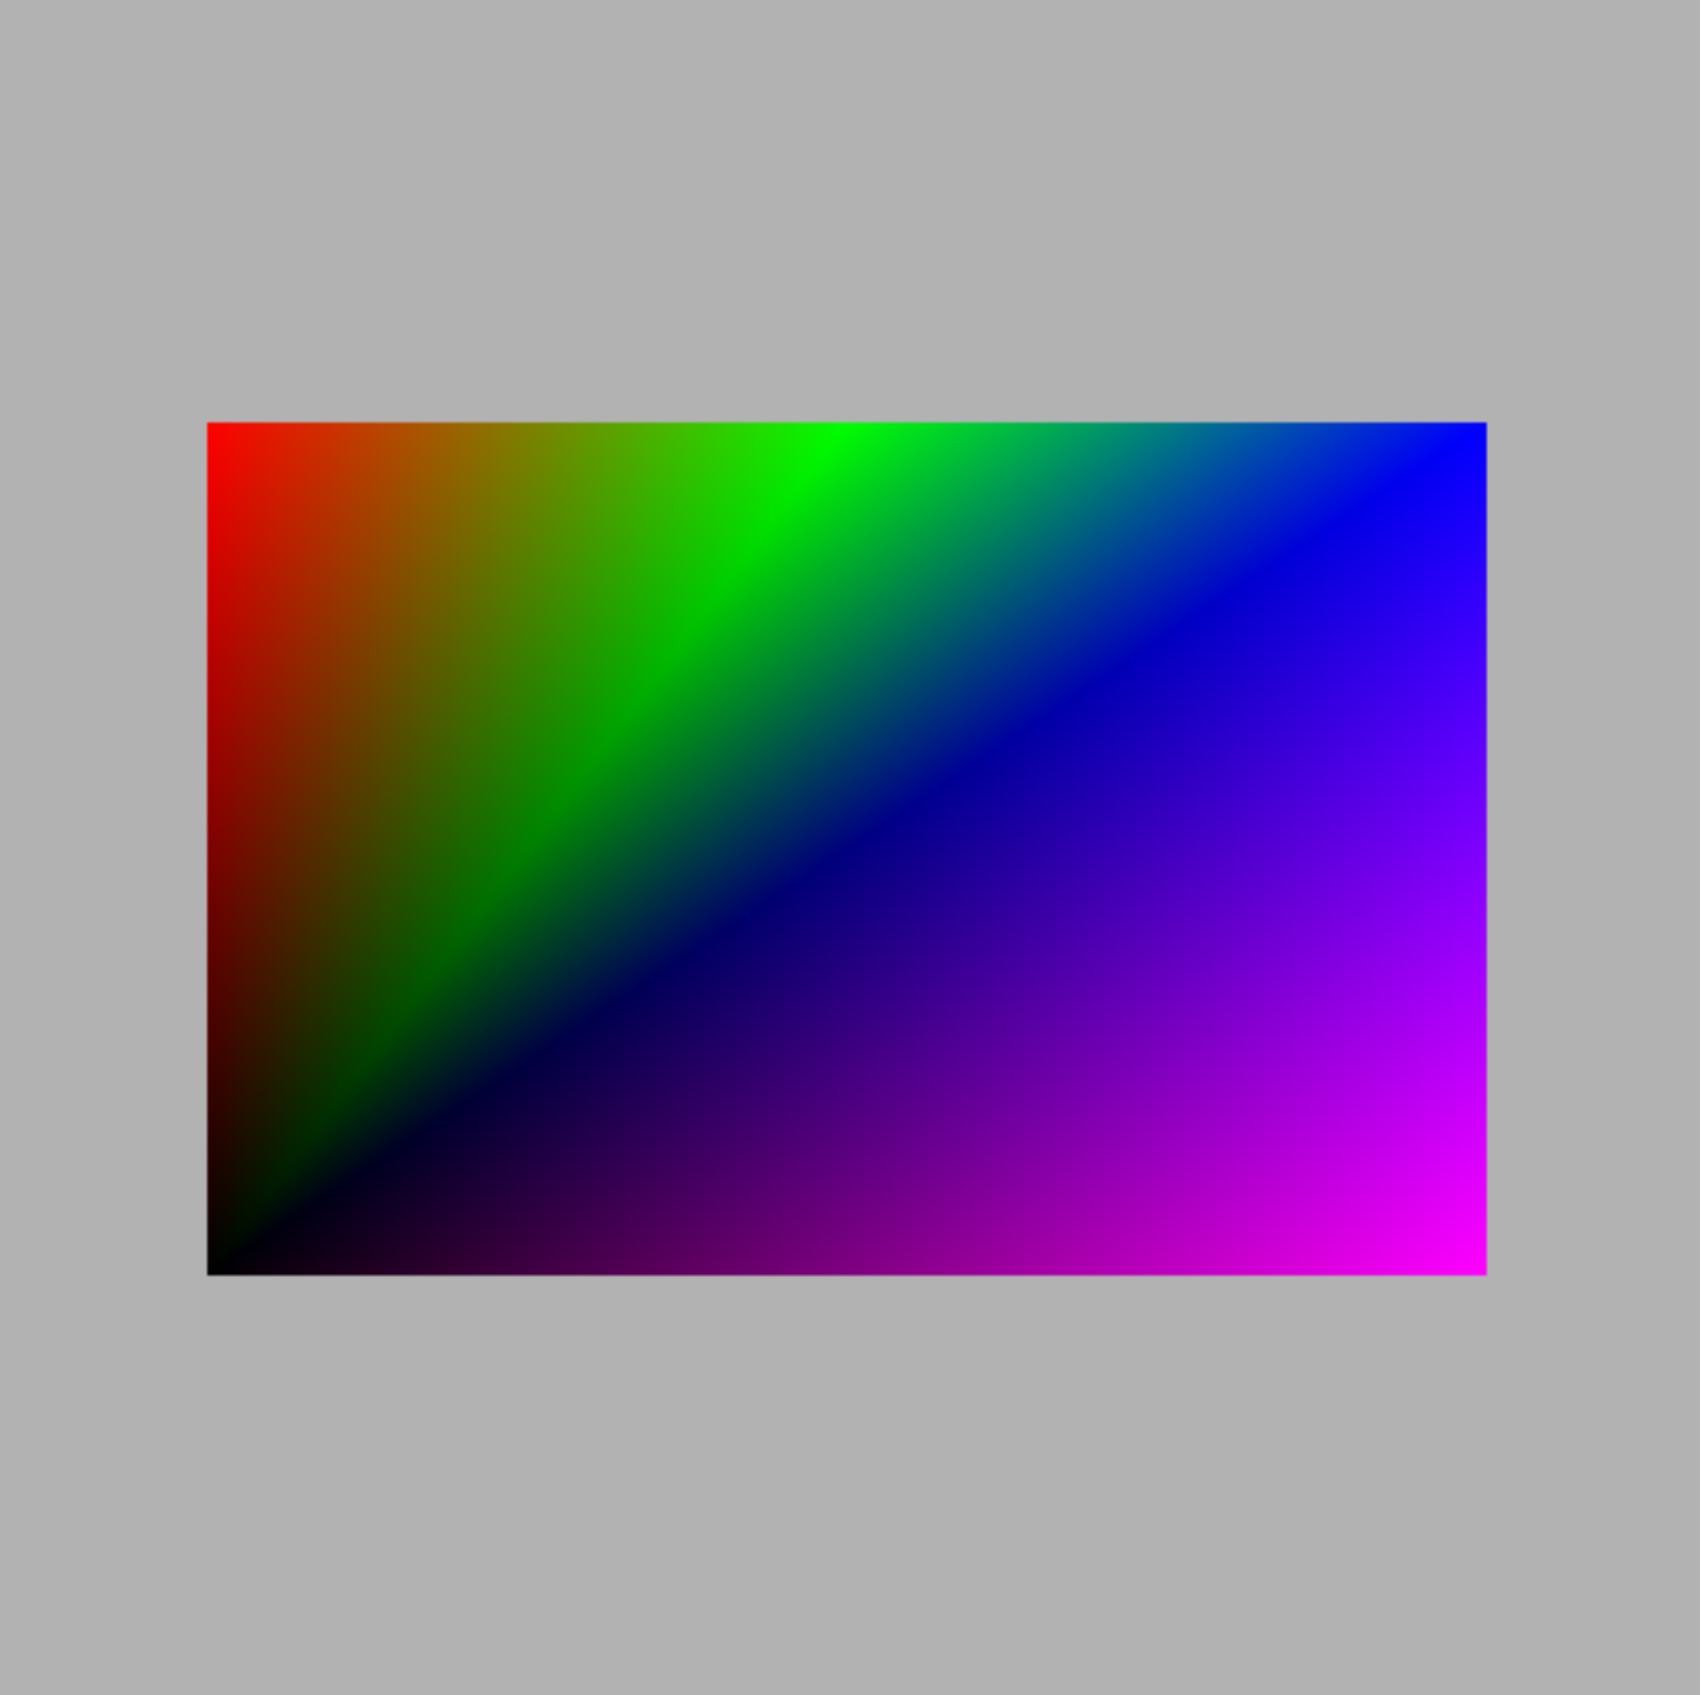
\includegraphics[width=1.0\textwidth]{Image_3}
\subsection{LINES}

\includegraphics[width=1.0\textwidth]{Image_4}
\subsection{TRIANGLES}
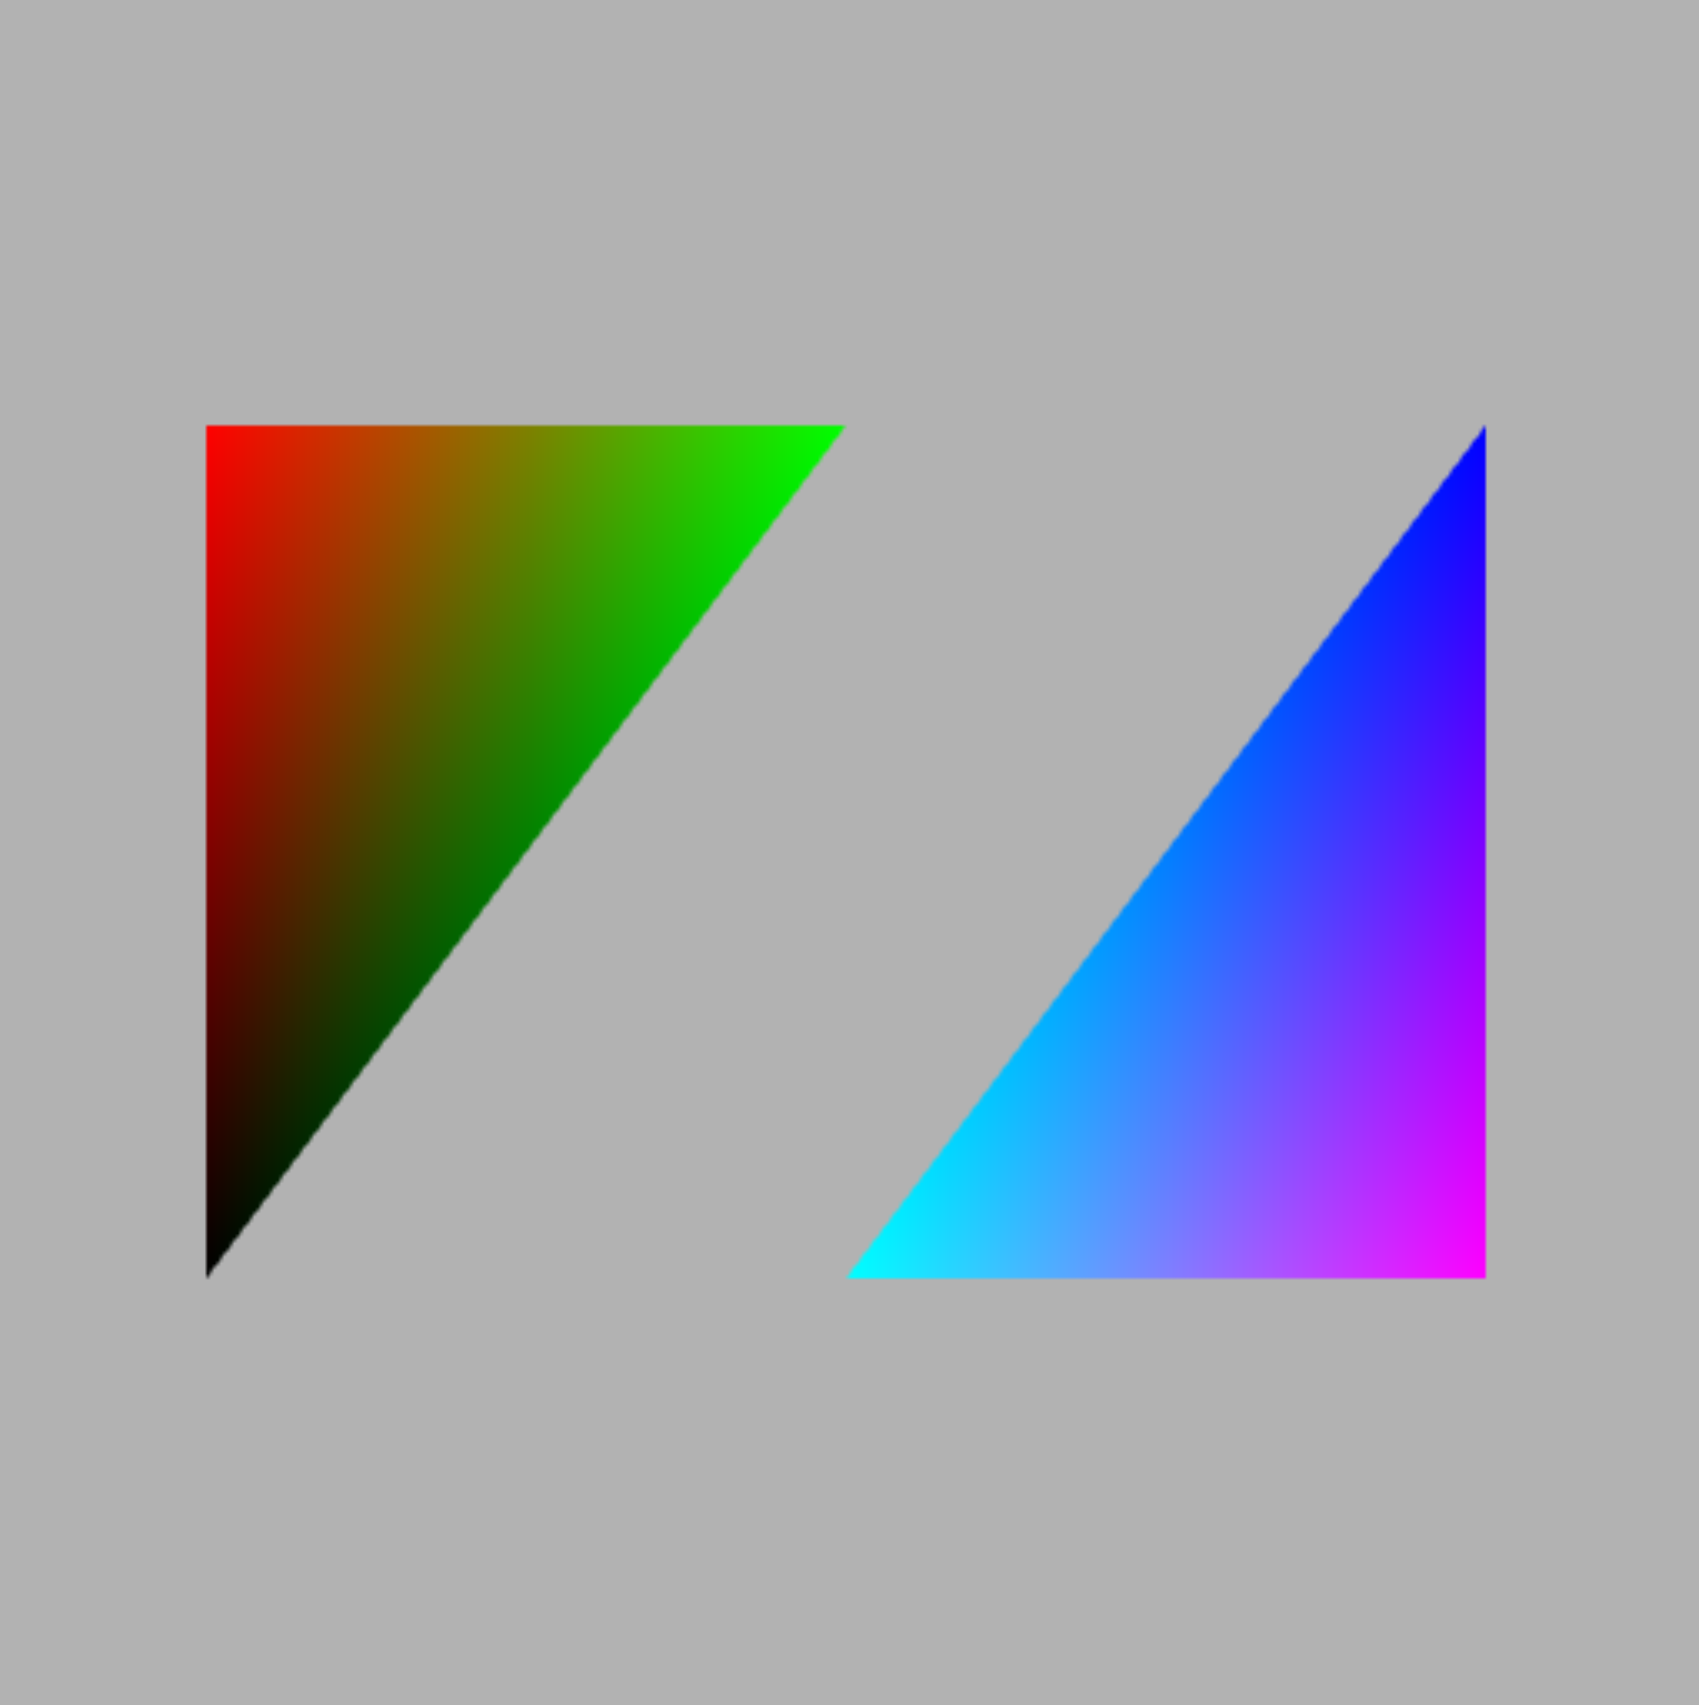
\includegraphics[width=1.0\textwidth]{Image_5}
\subsection{TRIANGLE FAN}

\includegraphics[width=1.0\textwidth]{Image_6}
\part{Question Six: Shading Language}
\section{Question}
In each case, name the built-in variable in the shading language.
\subsection{ A vertex must be assigned to this variable}
\subsection{Answer}
gl Position
\subsection{ A value can optionally be assigned to this variable to set the size of graphic that is used to display a point.}
gl PointSize
\section{Answer}
\part{Question Seven: Projection Transformations}
\section{Question}
What we call a projection transformation and have used in transforming vertices in our scenes is not actually a projection: it does not flatten the scene into two dimensions. Why is the scene left in three dimensions to be passed on to the fragment shader?
\section{Answer}
Because objects are not visible if they are farther away from the viewer then objects which are behind, or Depth Checking.
\part{Question Eight: Lighting Geometry}
\section{Question}
This question is about the geometry used to help compute the three kinds of shading: ambient, diffuse, and specular. When we computed shading, there were three main geometric components we used: vector from a point on a surface to the camera; vector from a point on a surface to the light source; vector normal to the surface. However, some of the shading types might use only some of these geometric components. Some might use none. This question asks you to tell for each geometric component, which kind of shading uses that component when being computed.
\subsection{Notes}
This part confuses me because there are only three shading methods to choose from I would want to just put all three for each one but I don't think I will.
\subsection{Which of the three kinds of shading depend on the direction to the camera?}
\subsection{Answer}
Specular depends on the direction of the camera.
\subsection{ Which of the three kinds of shading depend on the direction to the light source?}
\subsection{Answer}
Diffuse depends on the direction of the light source.
\subsection{ Which of the three kinds of shading depend on the normal to the surface?}
\subsection{Answer}
This will be the Ambient Lighting
\part{Question Nine: Texture Sampling Modes}
\section{Question}
\section{Answer}
\part{Question Ten}
\section{Question}
What feature when using images for textures in OpenGL makes use of reduced size images in areas where the texture image is larger than the area being covered?
\section{Answer}
You can use the mipmap feature to use a reduced size image texture.
\end{document}